% #############################################################################
% This is Chapter 1
% !TEX root = main.tex
% #############################################################################
% Change the Name of the Chapter i the following line
\fancychapter{Introduction}
\clearpage
% The following line allows to ref this chapter
\label{chap:chap001}
\noindent

This section presents the work motivation, goals and contributions achieved so far in the context of my research program.
The work described in this document started in September of 2015, before and during my Master Thesis~\cite{calisto2017mimbcdui}, founded by a research grant from \ac{FCT}.
The funding was provided under the \ac{RD} Units Strategic Plan - 2013/2015 - \ac{OE}, with the \href{https://www.fct.pt/apoios/projectos/consulta/vglobal_projecto.phtml.en?idProjecto=147329&idElemConcurso=8999}{UID/EEA/50009/2013} reference.
The official starting date of my \ac{PhD} program in \ac{CSE} at \ac{IST} of \ac{UL} is September of 2018 and since January of 2020 that my work has been funded by \ac{FCT} with the grant PD/BD/150629/2020 reference.

\section{Motivation}
\label{sec:sec001001}

Breast cancer is the second leading cause of death from cancer in women~\cite{doi:10.3322/caac.21492}.
However, early detection and treatment can considerably improve results~\cite{Seely2018, doi:10.1002/cncr.32859, 10.1093/jnci/djaa080}.
Consequently, large-scale of screening programs are implemented worldwide.
The majority of medical and governmental organizations recommend screening for all women starting between the ages of 40 and 50~\cite{Oeffinger2015, Koczkodaj2019}.
In Europe, over 400,000 new female cases are estimated to have risen each year~\cite{Dafni2019}.

Despite the extensive adoption of screening exams, interpretation of these images remains challenging.
The accuracy achieved by clinical experts in cancer detection varies widely (Figure~\ref{fig:fig016}), and performance of even the best clinicians leaves room for improvement~\cite{KIM2020e138, 10.1001/jamainternmed.2015.5231}.
For instance, the \acp{FP}\footnotemark[1] can lead to anxiety of the patient~\cite{10.1001/jamainternmed.2014.981}, avoidable follow-ups and unnecessary procedures of invasive diagnostics.
On the other hand, the \acp{FN}\footnotemark[2] are even more severe since the exam misdiagnoses a patient who has the disease~\cite{doi:10.1056/NEJMe1912943}.
During screening, the missing cancers may not be identified until they are more advanced and less agreeable to treatment~\cite{Houssami2017}.

%%%%%%%%%%%%%%%%%%%%%%%%%%%%%%%%%%%%%%%%%%%%%%%%%%%
\begin{figure}[ht]
\centering

\includegraphics[width=\textwidth]{images/fig016}
\caption{Proportions of breast cancer patients with missing cases and distribution among screened patients. Between 1 in 2 women have dense breasts and there are approximately 50\% chance of missing a cancer in dense breasts. Image from \protect\href{https://densitas.health/about}{densitas.health} in November 2020.}
\label{fig:fig016}
\end{figure}
%%%%%%%%%%%%%%%%%%%%%%%%%%%%%%%%%%%%%%%%%%%%%%%%%%%

%%%%%%%%%%%%%%%%%%%%%%%%%%%%%%%%%%%%%%%%%%%%%%%%%%%
\footnotetext[1]{False-Positive: when the screening result looks abnormal even though no cancer is actually present. Abnormal screening results often require extra testing to find out if the change is cancer. The \ac{FP} results are more common in women who are younger, have dense breasts, have had breast biopsies, have breast cancer in the family, or are taking estrogen.}
%%%%%%%%%%%%%%%%%%%%%%%%%%%%%%%%%%%%%%%%%%%%%%%%%%%

%%%%%%%%%%%%%%%%%%%%%%%%%%%%%%%%%%%%%%%%%%%%%%%%%%%
\footnotetext[2]{False-Negative: when the screening result looks normal even though breast cancer is present. Women with dense breasts are more likely to get \ac{FN} results. The \ac{FN} cases can give women a false sense of security, thinking that they don’t have breast cancer when in fact they do.}
%%%%%%%%%%%%%%%%%%%%%%%%%%%%%%%%%%%%%%%%%%%%%%%%%%%

The introduction of \ac{AI} in the medical workflows may be uniquely poised to help with this challenge~\cite{McKinney2020}.
Studies have demonstrated the ability of \ac{AI} to meet the human's performance on various clinical tasks~\cite{Topol2019, info:doi/10.2196/10010}.
As a lack of medical professionals threatens the adequacy and availability of clinical services worldwide~\cite{doi:10.1002/j.2051-3909.2012.tb00169.x, rimmer2017radiologist}, the scalability of \ac{AI} could improve to higher care.

In the medical imaging domains, \ac{AI} has the potential to improve visual diagnostic accuracy~\cite{Tschandl2020}.
\ac{AI}-based triage and decision support could assist readers, such as radiologists, in managing clinical workflows and improving their performance~\cite{doi:10.1148/ryai.2020190208}.
Most recent works have been predicted on comparisons of the diagnostic accuracy of \ac{AI} systems with clinicians~\cite{He2019, 10.1145/3313831.3376290}.
Furthermore, recent studies, in breast cancer, demonstrate that AI for diagnostic is equivalent or even superior to human experts in medical imaging under experimental conditions~\cite{Ribli2018, McKinney2020}.
This competitive view of AI is evolving based on studies suggesting that a more promising approach is an \ac{HAII}~\cite{10.1145/3313831.3376807, 10.1145/3290605.3300233, 10.1145/3411286, 10.1145/3313831.3376301}, with techniques that improve the interaction between humans and machines.

The role of \ac{HAII} in healthcare delivery the appropriate settings in which it can be applied, and its impact on the quality of care have yet to be evaluated~\cite{Tschandl2020}.
There have been several attempts at addressing the effects of \ac{HAII} across multiple workflows and different levels of clinical expertise~\cite{doi:10.1148/radiol.2019182627, doi:10.1148/ryai.2020200057}.
However, the use case of breast cancer diagnosis to address the effects from varied representations of \ac{AI}-based supported by intelligent agents is still scarce.
This explains why it is an open topic research, and the motivation behind the proposed research of this thesis.

\section{Objectives}
\label{sec:sec001002}

The goal of this thesis is the study, design and development, as well as evaluation of novel \ac{AI}-based visual representations~\cite{https://doi.org/10.13140/rg.2.2.29816.70409} supported by intelligent agents for medical imaging diagnosis.
For the purpose of this thesis, recent achievements~\cite{Tschandl2020, 9098470, MAICAS2019101562} are built in the accuracy of intelligent agents.
To address the effects of varied visual representations, the intelligent agents are applied for the breast cancer domain across different levels of medical expertise and multiple clinical workflows.
Chapter~\ref{chap:chap002} presents a brief description of the medical imaging background and the current workflow that clinicians use for acquiring and read the medical imaging data.
Shortly, the idea is to provide information concerning the rich opportunities available for research and development of intelligent agents in this medical workflow.

The rise of \ac{DL} for \ac{AI}-assistance in medical decision-making has created a strong need for large amounts of labeled data~\cite{10.1145/3313831.3376290}.
Frequently, the ground-truth labels required to develop supervised \ac{ML} algorithms~\cite{Yue_2020_CVPR} that are not given in the raw data.
Such settings require the expertise from medical professionals for manual data labelling.
In Chapter~\ref{chap:chap003}, this document provides a literature review and recent development in the \ac{HCI} community concerning the topic of \ac{AI}-assistance in medical decision-making.

\clearpage

Despite the promise of assisting clinicians in the decision-making process, there are two initial challenges~\cite{hugo2020si} that this thesis aims to cover: (i) the lack of available and curated medical data to be consumed by the \ac{AI} algorithms; and (ii) the fact that medical professionals often find it challenging to understand how an \ac{AI} system transform their initial input into a final decision.
Hence, two directions are followed.
The first direction tries to solve the lack of available and curated medical data by developing a framework~\cite{https://doi.org/10.13140/rg.2.2.16086.88649, calisto2019midaaiarfuv} to annotate, as well as to visualize masses and microcalcifications of breast cancer lesions in a multimodality\footnotemark[3] strategy~\cite{https://doi.org/10.13140/rg.2.2.14792.55049}.
The second direction is focused on enabling clinicians to understand existing medical data and its importance to the \ac{AI} algorithms.
In Chapter~\ref{chap:chap004}, the document will address these two direction goals.

%%%%%%%%%%%%%%%%%%%%%%%%%%%%%%%%%%%%%%%%%%%%%%%%%%%
\footnotetext[3]{Multimodality: diagnostic technique for the patient treatment via: (1) \ac{MG}, both \ac{CC} and \ac{MLO} views; (2) \ac{US}; (3) \ac{MRI}; and (4) text. The considered text modalities are, for instance, report information, personal history, family history, age, among others.}
%%%%%%%%%%%%%%%%%%%%%%%%%%%%%%%%%%%%%%%%%%%%%%%%%%%

Visualization support of multi-modal images and \ac{AI} techniques can provide improvements and insights in the breast screening workflow~\cite{https://doi.org/10.13140/rg.2.2.25412.68486}.
The goal of Chapter~\ref{chap:chap005} is to evaluate the impact for the introduction of these techniques in the context of the breast cancer diagnosis using an intelligent agent.
Specifically, Chapter~\ref{chap:chap005} focus on how multimodality and \ac{AI}-assistance could add value to the medical workflow in an \ac{UCD} process.
The answer of the thesis to this problem include usage and acceptance by clinicians and the improvement of workflow efficiency and quality, as well as reduction and prevention of errors and variability of diagnosis.

Chapter~\ref{chap:chap006} provides the clinicians' evaluation and results for several high-level goals, namely:
(a) understand clinicians' response to the \ac{AI}-assistance;
(b) find how they interact (and accept) with these systems; and
(c) discover how \ac{AI}-assistive affects the \ac{UX} of clinicians.
In this Chapter~\ref{chap:chap006}, the thesis broadly informs the literature in \ac{HCI} and \ac{AI} (\ac{HAII}) by examining what radiologists need when using \ac{AI}-powered image diagnostic, the practices they adopt while using diagnostic tools, and how these diagnostic tools affect end-user attitudes towards the underlying \ac{AI} algorithms.

A clinically oriented intelligent agent system can be achieved by mimicking the medical diagnosis and look for the presence of patient relevant clues in breast cancer images.
However, medical clues such as diagnosing dense breast patients, are difficult to read.
This approach ({\it i.e.}, \ac{HAII} that brings Human and \ac{AI} together), tend to be more easier for clinicians and leading to better patient results.
Chapter~\ref{chap:chap007} discuss the importance, as well as pros-and-cons for the introduction of intelligent agents in the medical imaging workflow.
As discussed in Chapter~\ref{chap:chap007}, several goals have been accomplished so far.
Nevertheless, work is still in progress and some goals have not been accomplished yet.

Finally, Chapter~\ref{chap:chap008} provides a direction to the most relevant future milestones.
The milestones are addressed in Chapter~\ref{chap:chap008} and some ideas on how to deal with them.
Different type of functionalities, as well as best way to communicate the agent results will be further investigated.
Combining functionalities and communication has not yet been investigated and will be addressed in future work.

\noindent
The approach towards these goals was divided in four parts (Figure~\ref{fig:fig017}) by showing the thesis problems and respective associated contributions:

\hfill

%%%%%%%%%%%%%%%%%%%%%%%%%%%%%%%%%%%%%%%%%%%%%%%%%%%
\begin{figure}[ht]
\centering
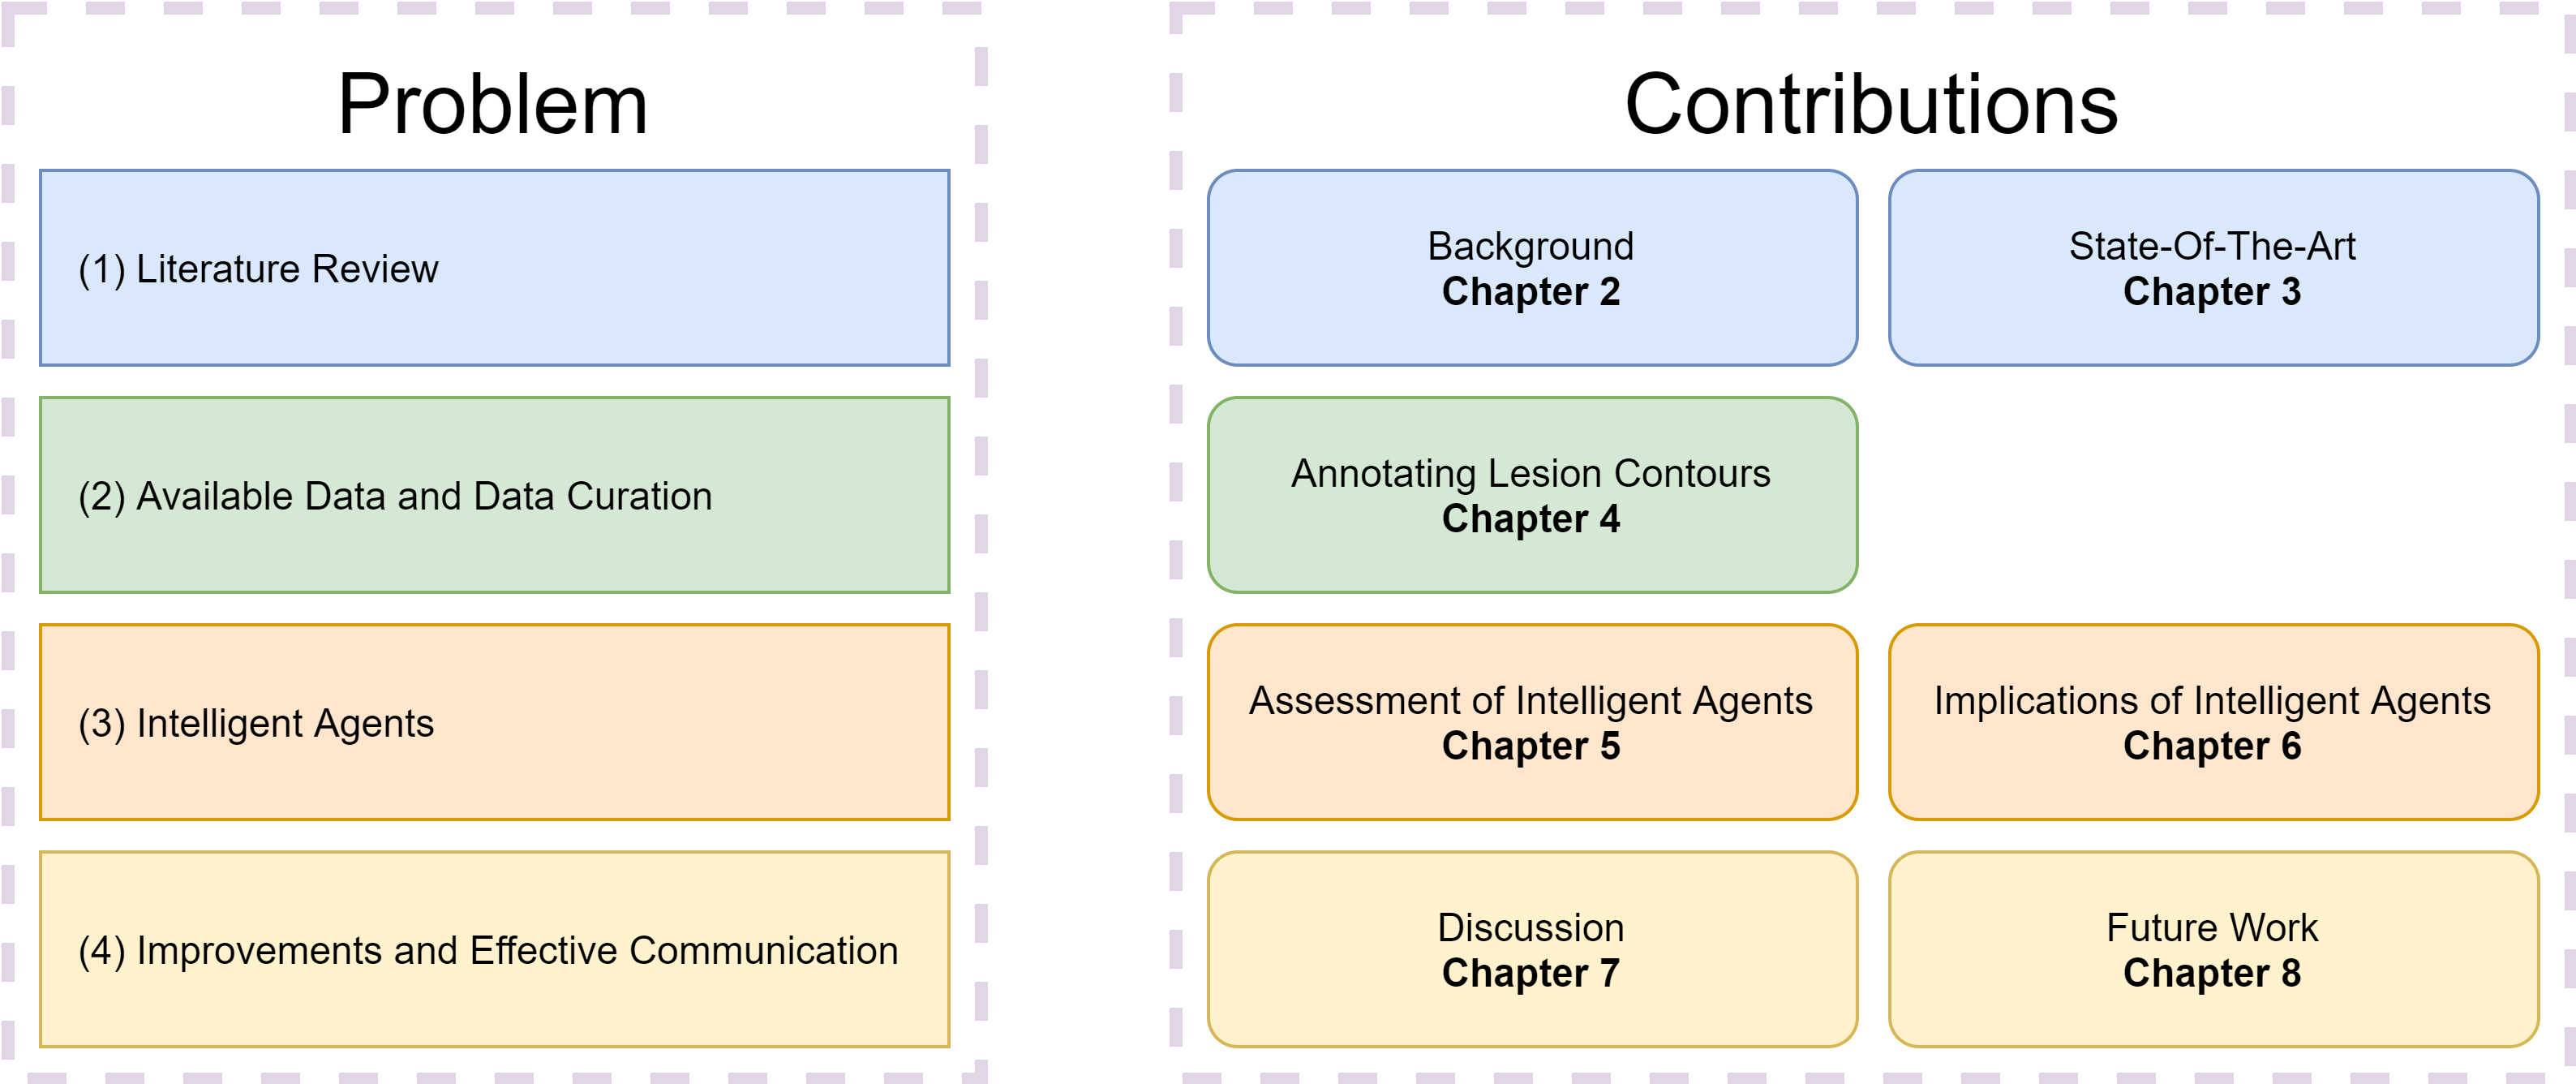
\includegraphics[width=\textwidth]{images/fig017}
\caption{[DOI: \protect\href{https://www.doi.org/10.13140/RG.2.2.14314.95685/1}{10.13140/RG.2.2.14314.95685/1}] Thesis problem and contribution~\cite{https://doi.org/10.13140/rg.2.2.14314.95685/1} relations. In this research, four scientific problems were addressed: (1) mitigating the bias between the clinical background of the medical imaging workflow and the related work of intelligent agents among the research communities; (2) developing a framework for annotating lesion contours to cover the lack of available and curated medical data problem; (3) the problems of assessment and implications of intelligent agents in the medical imaging workflow; and (4) the need for functionality improvements and effective communication of the intelligent agents.}
\label{fig:fig017}
\end{figure}
%%%%%%%%%%%%%%%%%%%%%%%%%%%%%%%%%%%%%%%%%%%%%%%%%%%

Several contributions are solving each problem (Figure~\ref{fig:fig017}) addressed in this thesis.
Although this document focus on the thesis main goals and contributions, one important objective of the document is to provide information concerning the medical imaging background and review of the literature for \ac{HCI} related work.
Thereafter, Chapter~\ref{chap:chap002} and Chapter~\ref{chap:chap003} are aiming to improve the understating of clinicians, researchers, engineers and policy makers in developing robust and effective data-driven interventions across the breast cancer domain.
In problem one, the literature review was stated as a problem and the respective contributions are present in this two chapters.
Moreover, problem four (covered by Chapter~\ref{chap:chap007} and Chapter~\ref{chap:chap008}) discuss and debate the achieved contributions.
In the end, it conclude the clinicians' needs for functionality improvements and effective communication of the intelligent agents, as well as the future work ahead of this thesis.
However, to simplify the central contributions, the next section (Section~\ref{sec:sec001003}) will just list the main contributions to solve problem two (covered by Chapter~\ref{chap:chap004}) and three (covered by Chapter~\ref{chap:chap005} and Chapter~\ref{chap:chap006}), respectively.

This thesis is one of the first contributions to address the above list of problems.
The effort to address each problem to the respective set of contributions, does not rely on any capacity or exercise in futuristic imagination.
Rather, the document aim to clarify the extent in which Humans and \ac{AI} techniques can be put under the evocative rubric of ``\ac{HAII}'' to improve the breast cancer diagnosis.

\clearpage

\section{Contributions}
\label{sec:sec001003}

The main contributions achieved so far are the following:

\begin{enumerate}
\item The design of an advanced visual interface to provide available and curated medical data for the annotation of lesion contours (masses and microcalcifications) on a multimodal strategy of the breast cancer diagnosis; ({\bf Chapter~\ref{chap:chap004}})
\begin{enumerate}[label*=\arabic*.]
\item The visualization of the two main types of breast lesions in \ac{MG}, \ac{US} and \ac{MRI} modalities of medical imaging;
\item Insights from the field comparison of single-modality {\it vs} multi-modality for screenings of breast cancer diagnosis with 31 clinicians and 566 images;
\end{enumerate}
\item Integration of several \ac{AI} techniques, using \acp{DNN}, to support automatic and reliable classification in medical imaging; ({\bf Chapter~\ref{chap:chap005}})
\item Development of a novel \ac{AI} system based on intelligent agents to support a multi-modal imaging strategy; ({\bf Chapter~\ref{chap:chap005}})
\begin{enumerate}[label*=\arabic*.]
\item User study findings of 45 clinicians comprising nine clinical institutions;
\item List of design recommendations for visualization to support breast screening radiomics;
\item Evidence from the impact of multimodality and \ac{AI}-assisted strategy in diagnosing and severity classification of lesions;
\item Evaluation results of a proof-of-concept prototype for the \ac{AI}-assisted condition;
\end{enumerate}
\item Introduction of an \ac{AI}-assisted system in the medical imaging workflow which provides an automated diagnostic based on the developed \ac{DL} methods; ({\bf Chapter~\ref{chap:chap006}})
\begin{enumerate}[label*=\arabic*.]
\item Quantitative and qualitative results to measure:
\begin{enumerate}[label*=\arabic*.]
\item How receptive are the clinicians to the introduction of \ac{AI}-assisted medical imaging and agent-based systems;
\item How they accept and interact with these systems;
\item How \ac{AI}-assistance influence the \ac{UX} perception in the clinical context;
\end{enumerate}
\item Introduction and study for the impact of an intelligent agent into a real-world case study of 45 clinicians from nine institutions;
\item Accuracy comparison (measured in terms of \acp{FP} and \acp{FN} metrics) of \ac{AI}-assisted results;
\item Study the impact of several design techniques on the expectations and satisfaction of the clinicians in different groups of medical professional experience.
\end{enumerate}
\end{enumerate}

\clearpage

\section{Future Objectives}
\label{sec:sec001004}

Several objectives have been accomplished so far, as discussed in the two (Section~\ref{sec:sec001002} and Section~\ref{sec:sec001003}) previous sections.
However, work is still in progress and some goals have not been accomplished yet.
This section provides a direction to the most relevant future milestones, which are addressed in Chapter~\ref{chap:chap008}, as well as some ideas on how to deal with them.

The last part of the thesis main contributions (Chapter~\ref{chap:chap006}) consists in addressing implications for the introduction of intelligent agents as a clinical problem.
This means taking into account that \ac{AI} algorithms are not perfect, as well as what are the clinicians' needs concerning the provided information coming from the agents.
The implications are several and the future objectives must take into account what are the current hazards of each agent to fulfill the respective use case for a better patient diagnostic.
New agent functionalities must be improved to achieve a more effective communication of the agent.
Also, although this document have focused mainly on the development of intelligent agents, there is still room for improvements and further work to be done.

One important issue that the thesis covers is the lesion annotation (Chapter~\ref{chap:chap004}) so that the \ac{AI} algorithms have available and curated data.
On the one hand, the quality of annotation depends on the clinician’s experience.
On the other hand, it also depends on the number of study cases, such as:
(i) annotations made manually by clinicians useful to extract functionalities like lesion contours;
(ii) shape and margins that can be used in the computation of lesion segmentation; and
(iii) classification made by intelligent agents.
In this work, several new functionalities must be integrated~\cite{hugo2020si} to support a higher and better annotation process.
Therefore, the introduction of the following four new functionalities is important:
(1) Recorded View ;
(2) Temporal Comparison View ;
(3) Coordinated View ; and
(4) 3D Module View.
The functionalities aim to lower the annotations time and to improve its precision.

Overstated expectations about \ac{AI}~\cite{https://doi.org/10.13140/rg.2.2.25412.68486, calisto2019midaaiarfuv} and unknown levels of assertiveness decrease user acceptance and adoption of clinical systems.
In particular, when expectations are not met, clinicians' levels of trust will decrease during time~\cite{Kocielnik:2019:YAI:3290605.3300641}.
Another future objective is to study and understand how the level of assertiveness~\cite{10.1145/3311350.3347162, pacheco2019alignment}, will impact the clinicians' decision-making during diagnostic.

In these intelligent agents, most functionalities are seen by clinicians with limited computational knowledge as `black boxes'~\cite{10.1145/3313831.3376807}.
A future objective is enabling clinicians to explore and understand the \ac{AI} results.
In this work, such goal can be achieved by the integration of the \ac{XAI} topic with different setups.
For instance, {\it Agent A} explains the classification results of the patient, while {\it Agent B} explains the segmentation results.
Indeed, they are different \ac{DNN} methods.
The first agent ({\it i.e.}, {\it Agent A}), can be explaining the results coming from \ac{CNN} models ({\it e.g.}, DenseNet~\cite{Huang_2017_CVPR}, ResNet~\cite{He_2016_CVPR}, between others~\cite{10.1117/12.2549103}) as image classifiers.
On the contrary, the second agent ({\it i.e.}, {\it Agent B}), can be explaining the results coming from models ({\it e.g.}, HyperDense-Net~\cite{8515234}, U-Net~\cite{10.1007/978-3-319-24574-4_28} or different ones~\cite{10.1007/978-3-030-46640-4_23}) for image segmentation.

\clearpage

The only intelligent agent described in this document (Chapter~\ref{chap:chap005} and Chapter~\ref{chap:chap006}) use an image classifier ({\it i.e.}, DenseNet~\cite{Huang_2017_CVPR}), that is limited for image classification.
Thus, clinicians cannot understand the decision of such system.
For example, when the system fails, it is difficult to know the reason.
One \ac{DNN} method was integrated with the intelligent agent to classify the cancer severity of each patient, but these medical clues have not yet been used for an automatic lesion segmentation.
Instead, to output the heatmaps (Chapter~\ref{chap:chap005} and Chapter~\ref{chap:chap006}), we are using the manual annotations by computing the circularity of the lesion~\cite{DALILA2017749} and color-related to the computed severity.
However, clinicians do not diagnose patients solely using image information.
As described in Chapter~\ref{chap:chap002}, different patient aspects are considered before performing the final diagnosis.
In order to develop a fully clinically oriented agent it will be necessary to address more methods and other clinical co-variables.

\section{List of Publications}
\label{sec:sec001005}

The work developed in this thesis was published in conference and journal papers. The following sections will list the set of publications published and/or under revision (but accepted) until now.

\subsection{Conference Papers}
\label{sec:sec00100501}

\begin{enumerate}
\item Francisco M. Calisto, Alfredo Ferreira, Jacinto C. Nascimento, and Daniel Gonçalves. 2017. Towards Touch-Based Medical Image Diagnosis Annotation. In Proceedings of the 2017 ACM International Conference on Interactive Surfaces and Spaces (ISS '17). Association for Computing Machinery, New York, NY, USA, 390–395. DOI: \href{https://doi.org/10.1145/3132272.3134111}{https://doi.org/10.1145/3132272.3134111}
\item Francisco Maria Calisto, Nuno Nunes, and Jacinto C. Nascimento. 2020. BreastScreening: On the Use of Multi-Modality in Medical Imaging Diagnosis. In Proceedings of the International Conference on Advanced Visual Interfaces (AVI '20). Association for Computing Machinery, New York, NY, USA, Article 49, 1–5. DOI: \href{https://doi.org/10.1145/3399715.3399744}{https://doi.org/10.1145/3399715.3399744}
\end{enumerate}

\subsection{Journal Papers}
\label{sec:sec00100502}

\begin{enumerate}
\item Francisco Maria Calisto, Carlos Santiago, Nuno Nunes, and Jacinto C. Nascimento. Radiomics Hope or Hype? An HCI Assessment of AI-Assisted Medical Imaging for BreastScreening. International Journal of Human-Computer Studies. [UNDER REVISION]
\end{enumerate}